\documentclass[12pt,MSc,twoside]{muthesis}
% The regulations say that 12pt should be used
% Change the MSc option to MPhil, MRes or PhD if appropriate

\usepackage[utf8]{inputenc}
\usepackage[T1]{fontenc}
\usepackage{verbatim}
\usepackage{graphicx}
\usepackage{url} % typeset URL's reasonably
\usepackage{amsmath}
\usepackage{xcolor}
\usepackage{listings}
\usepackage{hyperref}
\usepackage[acronym, toc]{glossaries}
\usepackage[english]{babel}
\usepackage{csquotes}
\usepackage{booktabs}
\usepackage[
backend=biber,
style=alphabetic,
sorting=ynt
]{biblatex}

\usepackage{pslatex} % Use Postscript fonts

\lstset{
    basicstyle=\scriptsize,
    frame=single,
    breaklines=true,
    postbreak=\raisebox{0ex}[0ex][0ex]{\ensuremath{\color{black}\hookrightarrow\space}}
}

% Uncomment the next line if you want subsubsections to be numbered
%\setcounter{secnumdepth}{3}
% Uncomment the next line if you want subsubsections to be appear in
% the table of contents
%\setcounter{tocdepth}{3}

% Uncomment the following lines if you want to include the date as a
% header in draft versions
\usepackage{fancyhdr}
\pagestyle{fancy}
\lhead{}  % left head
\chead{Draft: \today} % centre head
\lfoot{}
\cfoot{\thepage}
\rfoot{}

\makeglossaries

\newglossaryentry{APU}
{
    name=APU,
    description={Accelerated Processing Unit, an AMD effort to produce a single chip that integrates both a CPU and a GPU}
}

\newglossaryentry{accelerator}
{
    name=accelerator,
    description={"Hardware device or capability that enables accelerated computation on data-parallel workloads'' \cite{Microsoft2013}, that works in conjunction with the CPU}. Also referred to as a ``coprocessor''
}

%\newglossaryentry{API}
%{
%    name=API,
%    description={Application Programming Interface, set of functions related to each other that act as a building block for other programs}
%}

\newglossaryentry{core}
{
    name=core,
    description={Hardware processing unit, capable of executing instructions read from a program}
}

\newglossaryentry{compute unit}
{
    name={compute unit},
    description={In OpenCL, a work group executes on a compute unit, which is composed of one or more processing elements (cores) and local memory}
}

\newglossaryentry{data parallelism}
{
    name={data parallelism},
    description={A form of parallelism concerned with partitioning data over many cores, usually simple to implement and scalable wth higher numbers of cores~\cite{tsuchiyama2010opencl}}
}

\newglossaryentry{distributed computing}
{
    name={distributed computing},
    description={High-performance computing by communicating and coordinating between a considerable number of computers, using MIMD architectures}
}

\newglossaryentry{global work size}
{
    name={global work size},
    description={The total number of work-items that will execute a kernel function (i.e. a function issued by a host, in the form of a command, to be executed by a device) in OpenCL}
}

\newglossaryentry{GPGPU}
{
    name={GPGPU},
    description={General Purpose computing on Graphics Processing Units, the programming practice of using GPUs for computing not related with rendering of 3D graphics}
}

\newglossaryentry{heterogeneous}
{
    name={heterogeneous},
    description={A heterogeneous system (or heterogeneous architecture) is one composed of different types of processors and accelerators with different technical specifications}
}

\newglossaryentry{HPC}
{
    name={HPC},
    description={High-Performance Computing, a practice concerned with very efficient implementations of large scale computational problems}
}

\newglossaryentry{instruction-level parallelism}
{
    name={instruction-level parallelism},
    description={A form of parallelism concerned with low level processor techniques for issuing instructions concurrently}
}

\newglossaryentry{kernel}
{
    name={kernel},
    description={A small function that can be executed by a core}
}

\newglossaryentry{local work size}
{
    name={local work size},
    description={The number, usually accompanied by the dimensions, of work-items that compose a work-group in OpenCL}
}

\newglossaryentry{MIMD}
{
    name={MIMD},
    description={``Multiple Instruction, Multiple Data'', a class of architecture capable of coordinating between different cores to execute different instructions in parallel}
}

\newglossaryentry{memory latency}
{
    name={memory latency},
    description={The time spent in data transfers and copies between different memory types, e.g. from RAM to CPU registers or to a dedicated accelerator memory}
}

\newglossaryentry{multi-core}
{
    name=multi-core,
    description={Hardware component that integrates more than one core (processing unit) as part of its design and that is able to use them independently}
}

\newglossaryentry{NDRange}
{
    name=NDRange,
    description={An n-dimensional index space that describes how many work-items were created to execute kernels in OpenCL}
}

\newglossaryentry{OpenCL device}
{
    name={OpenCL device},
    description={In the context of OpenCL, a device is a collection of compute units.}
}

\newglossaryentry{PCIe}
{
    name={PCIe},
    description={Peripheral Component Interconnect Express, a currently leading hardware interface for connecting additional accelerators to a computer}
}

\newglossaryentry{pipeline parallelism}
{
    name={pipeline parallelism},
    description={A form of parallelism concerned with organising data streams and a series of tasks into a pipeline structure}
}

\newglossaryentry{processing element}
{
    name={processing element},
    description={The elements that compose an OpenCL compute unit, which is part of a device}
}

\newglossaryentry{SIMD}
{
    name={SIMD},
    description={``Single Instruction, Multiple Data'', a class of architecture capable of executing instructions on many data elements in parallel}
}

\newglossaryentry{shared memory}
{
    name={shared memory},
    description={Architectures capable of sharing the same memory space between their multiple processors}
}

\newglossaryentry{task parallelism}
{
    name={task parallelism},
    description={A form of parallelism concerned with partitioning (possibly different) operations and routines over many cores, usually requiring advanced load balancing techniques~\cite{tsuchiyama2010opencl}}
}

\newglossaryentry{thread}
{
    name=thread,
    description={The minimal representation of a set of instructions that can be executed by a computer, and be handled by the operating system scheduler}
}

\newglossaryentry{vectorisation}
{
    name=vectorisation,
    description={Vectorisation occurs when many elements of a vector are processed by one instruction of the processor concurrently}
}

\newglossaryentry{work-group}
{
    name={work-group},
    description={A set of work-items mapped to the same compute unit in OpenCL, that are able to share resources (e.g. memory)}
}

\newglossaryentry{work-item}
{
    name={work-item},
    description={An equivalent of a thread in OpenCL jargon}
}


%\newacronym{vpu}{VPU}{Vector Processing Unit}


\addbibresource{refs.bib}

\begin{document}
% Uncomment the following lines to leave out list of figures, tables
% and copyright until final printing
%\figurespagefalse
%\tablespagefalse

%\copyrightfalse

\title{Portable Performance for \\
  Heterogeneous Parallel Architectures}
\author{Arturo Isa\'i Castro P\'erpuli}
\principaladviser{Dr. Graham Riley}

\beforeabstract

\prefacesection{Abstract}
%\abstracttitle
% Single spacing can be turned on for the abstract
%
{\singlespacing

% NO MORE THAN 300!!!

Programming is difficult in a general sense. Tuning for parallel performance adds more complexity to a program. Complexity means more potential bugs and greater difficulty to introduce changes to existing code, reducing its maintainability. Coupling these observations with the fact that most programs today are designed for a particular piece of hardware means that current applications have a limited lifespan. 

As hardware continues to evolve, new and different products will continue to emerge. The current trends in computer architectures dictate that future hardware configurations will contain different kinds of chips, mixing their individual performance capabilities, both for maximising performance for existing programs, as well as for widening the range of applications that can be created to tackle problems where high performance is a decisive factor.

However, creating programs for these heterogeneous architectures with current programming models represents a formidable task. New performance portability techniques are needed. While custom versions of programs for specific architectures might always yield better results than programs made with these new techniques, the savings in terms of human effort are undeniable and could mean a much more viable application development life-cycle, with longer intervals between high performing versions.

The aim of the project is to explore cost-effective (in terms of time and human effort) ways to exploit parallelism targeting heterogeneous architectures with the same code base. In this report a case for the portability of performance is made and a research methodology is consolidated to evaluate approaches to performance portability.

}


\afterabstract

%\prefacesection{Acknowledgements}
%I would like to thank...
%\afterpreface

\printglossary

% These include the actual text
\chapter{Introduction -- CHANGES PENDING}
\label{cha:intro}

%\section{How to read this document}

The design of microprocessor technology has hit several ``walls'' in recent decades ~\cite{Collange2013}~\cite{borkar1999design}~\cite{2_sutter_2015}. These limits occur when a specific component of the chip cannot be improved further in the next generations, because of cost or physical constraints. As a result, the paradigm for achieving performance changed and the industry turned to \gls{multi-core} architectures (i.e. hardware that integrates more than one \gls{core}) to provide power-efficient and scalable computers \cite{flynn2005microprocessor}.

While CPU performance continues to be improved, an alternative is to use \glspl{accelerator}, i.e. additional hardware that, in addition to CPUs, can perform operations. These accelerators use more and simpler cores than CPUs and can better exploit fine-grained parallelism~\cite{borkar2007thousand}~\cite{Collange2013}.

These efforts result in varied chip designs, with different number, frequency and types of cores. This gives rise to \gls{heterogeneous} systems, computers that are composed of distinct combinations of processor components. The problem is that performance is not portable across architectures. New models of chips and accelerators are continuously created by manufacturers. Each chip may only be programmable with specific programming languages. Creating new versions of programs for each architecture becomes unfeasible for programmers.

The aim of this project is to evaluate and extend the work in \cite{dolbeau2013one}, which suggests a solution for the portability of performance. The idea is that good performance may be obtained across a range of heterogeneous architectures if the code is tuned so as not to fully exploit a particular architecture. Performance losses across heterogeneous systems are minimised, at the cost of not achieving ``peak'' performance on one architecture.

The project will make use of several types of machines that are composed of different kinds of accelerators. Specifically, the hypothesis will be evaluated with three OpenCL-compatible architectures: an Intel 24-core multi-socket CPU, an Nvidia 2496-core GPU and an Intel Xeon Phi 60-core accelerator. The architectures chosen provide different performance characteristics and implementations of the OpenCL standard.

% TODO

Other alternatives will optionally be surveyed, e.g. using libraries that achieve performance portability for heterogeneous architectures, like ArrayFire~\cite{malcolm2012arrayfire}, or implementing auto-tuning approaches~\cite{ganapathi2009case} (which can automatically get good performance). This is optional since it is not known if the libraries will work with the platforms available for experimentation. Auto-tuning approaches may prove too complex to implement in the available time.\\

\section{Aim}
\label{sec:aim}

Explore cost-effective (in terms of time and human effort) ways to exploit parallelism targeting heterogeneous architectures with the same code base.

\section{Objectives}

\begin{itemize}
\item Understand performance characteristics in heterogeneous architectures.
\item Provide implementations of an algorithm that exploit the performance of different architectures.
\item Evaluate a version of an implementation of an algorithm, able to extract performance from heterogeneous architectures with no code changes, against other architecture-specific implementations.
\item Evaluate if trading peak for generally good performance can achieve performance portability for heterogeneous architectures.

\section{Structure of Dissertation}

The following document is structured as suggested in the lecture notes of the COMP90990 course. Chapter~\ref{cha:back} presents a survey of relevant literature for the project. Current parallel hardware options are reviewed, along with available parallel programming models for creating suitable programs that can exploit these hardware options.

Chapter~\ref{cha:methodology} explains the approach this project will take to try to obtain good performance from heterogeneous parallel architectures on a given program, without making changes to the source code of the program. This approach is based on the work done in~\cite{dolbeau2013one}, as mentioned in this introduction. The choice of the program to consider and the methods for evaluating the results obtained will be discussed in this chapter as well.

All progress made as of time of writing on this project will be presented in Chapter~\ref{cha:exp1}, including some preliminary results from running existing versions of code that implement a chosen algorithm in some of the architectures available for experimentation.

Chapter~\ref{cha:conclusion} serves as a conclusion to this report, summarising the key concepts defined and points made during this project.

\end{itemize}

\chapter{Background}
\label{cha:back}

This chapter presents a survey of relevant literature for the project. In Section 2.1, Parallelism is discussed, along with the variety of parallel architectures and specific hardware components that are available for programmers to use in order to write high-performing programs. In Section 2.2, the programming models and languages that may be used to write these parallel programs are reviewed, with a focus on compatibility and portability of performance. In Section 2.3, an argument for the importance of portable performance is proposed.

\section{Parallelism and parallel architectures}

In this section, relevant concepts of parallelism and parallel architectures will be surveyed. A list of hardware component types capable of performing parallelism is also discussed.

The project discusses parallelism which, as explained in Chapter~\ref{cha:intro}, has become the norm when designing new hardware components for high performance. There are different kinds of parallelism that manifest when designing parallel programs. 

Data parallelism and task parallelism are two prominent examples\cite{subhlok1993exploiting}. Data parallelism considers partitioning a data stream between different cores, after which each core can process its data partition in parallel. In contrast, task parallelism deals with how the actual processing operations and routines can be partitioned among different cores.

Instruction-level parallelism refers to low-level techniques that are exploited by processors when executing programs, like out-of-order execution~\cite{hennessy2012computer}. While a viable source for performance, its relatively poor range of optimisations geared towards parallelism has prevented it from being the only method used for parallelism~\cite{goossens2013limits}.

Pipeline parallelism is another alternative used by both hardware and software components, dealing with how the processing of a data stream can be broken up into several stages and put through a pipeline mechanism. As data keeps flowing into the process, parallelism may be achieved~\cite{gordon2006exploiting}. A graphical example comparing data, task and pipeline parallelism in a single hypothetical application is shown in Figure~\ref{f:parallelism}.

\begin{figure}[!h]
\begin{center}
\centerline{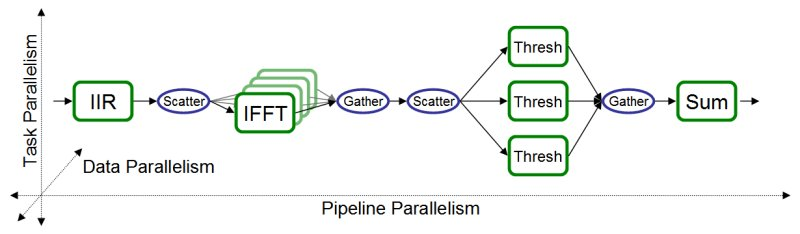
\includegraphics[width=\columnwidth]{img/parallelism}}
\caption[Example stream graph with parallelism axes.]{``Example stream graph with parallelism axes. Filters are denoted by green boxes and data-reorganization nodes are denoted by blue ovals. Pipeline parallelism is present between filters in the horizontal dimension, task parallelism in the vertical dimension, and data parallelism in the perceived depth dimension. Data parallelism is exploited only in IFFT. IFFT is stateless and can be data-parallelized by duplicating the filter (duplicates denoted by lighter boxes)'', as explained by ~\cite{1_gordon_thies_li_sung_zhang_wong_amarasinghe_2015}.}
\label{f:parallelism}
\end{center}
\end{figure}

Familiarity with the basics of computer architecture~\cite{hennessy2012computer} and Flynn's Taxonomy~\cite{flynn1966very}~\cite{tsuchiyama2010opencl} is assumed, which classifies parallel hardware according to its capabilities to execute parallel. In particular, concepts such as ``Single Instruction, Multiple Data'' (\gls{SIMD}) and ``Multiple Instruction, Multiple Data'' (\gls{MIMD}) are used throughout this document.

SIMD architectures refer to chips that are able to execute a single instruction in parallel on more than one data element. This can be achieved by specific instruction support on a single core, or by employing hardware with multi-core capabilities, among other approaches. MIMD architectures are composed of two or more components that can coordinate among themselves to execute different instructions on different data. MIMD examples can also include multi-core processors, but more complex approaches like clusters of many computers connected by a network also fit into this category.

Specific types of hardware components capable of processing will now be presented. These components are examples of parallel architectures that have been prominent in the history of parallel computing. 

\subsection{CPU}

CPUs have been at the forefront of the parallel hardware evolution, ever since major CPU manufacturers hit the ``power wall'' (i.e. the difficulty in dissipating heat from chips with high frequencies~\cite{flynn2005microprocessor}~\cite{2_sutter_2015}) in the early 2000's~\cite{flynn2005microprocessor}. At the same time, there is competition between specific CPU architectures from different vendors, each with their own characteristics and peculiarities that offer differences in terms of performance~\cite{Masoumzadeh2013}, e.g. the number and frequency of cores, the length of exploitable SIMD, etc. Even task-level parallelism is important in this regard, as some chips integrate cores with both low and high frequencies to provide further power savings in the interest of extending the battery life of mobile devices~\cite{zhu2013high}.

\subsection{GPU}

A Graphics Processing Unit (GPU) is an accelerator usually tasked with the rendering of 3D graphics, but also capable of general-purpose computing~\cite{Microsoft2013}. GPUs integrate many simple processing units that can be used in parallel for simple calculations. (e.g. basic arithmetic). The rendering of 3D graphics has its roots in linear algebra and the projections of 3D vectors in a 2D space~\cite{7_wikipedia_2015}. The algorithms for performing these projections are data-parallel and thus GPUs are used to cope with the performance needs of these projections~\cite{wu2011gpu}~\cite{8_wikipedia_2015}.

It was around the same time that multi-core chips became the norm (in the early 2000s~\cite{flynn2005microprocessor}) that there were developments regarding the use of GPUs for general purpose computing, a practice referred to as \gls{GPGPU} \cite{nickolls2010gpu}. Just like the case of CPUs, there are different vendors and models of GPUs, each with their own set of specifications.

Accelerators like GPUs are often connected through a bus interconnect in order to share data between the main memory (which shares some of its data with the CPU) and the device's own memory (used to share data with the processing units in the accelerator). However, data must eventually go through the main memory and the CPU for many critical operations. The time needed to transfer data from the main memory to the CPU and back (i.e. the main \gls{memory latency}) is faster than the memory latency from data transfers between accelerators and the main memory~\cite{daga2011efficacy}. This creates a bottleneck that limits the potential usefulness of accelerators~\cite{goddeke2007exploring} and reaffirms the importance of CPUs, in spite of their relative good parallel performance.

In the mobile world, graphics have become important and devices often feature low-power GPUs~\cite{cheng2011using}. The inclusion of cameras provides further opportunities for GPGPU~\cite{wang2013accelerating}~\cite{rister2013fast}, making real-time computer vision and image processing applications a reality at reasonable power consumption levels which provides extended battery life.

One development in GPU technology are Accelerated Processing Units ((\gls{APU}s). Initially developed by ATI, and then by AMD, it consists on a single chip that comprises both a CPU and a GPU on the same die, which provides less memory latency by eliminating the need of PCIe accesses~\cite{daga2011efficacy}. Since the Sandy Bridge architecture, Intel provides a very similar design in CPUs by incorporating Intel HD Graphics chips on the same die as well~\cite{yuffe2011fully}.

APUs are very popular on modern CPU designs and on video game consoles because of their relative low power-consumption and memory latency~\cite{9_wikipedia_2015}, with newer developments providing the CPU and GPU components with the same memory address space, preventing unnecessary data transfers between themselves~\cite{10_wikipedia_2015}.

\subsection{MIC}

A new approach to building accelerators has been proposed by Intel in 2010, in the form of the Intel Many Integrated Code (Intel MIC) architecture. It is based on work on the cancelled Larrabee~\cite{seiler2008larrabee} GPU-like architecture by Intel, originally announced in 2008. The Larrabee would include characteristics of both GPUs (support for 3D graphics using DirectX and OpenGL) and CPUs (composed by x86 cores that would benefit from the x86 instruction set and cache coherency among all cores)~\cite{seiler2008larrabee}.

The MIC architecture is composed of more and simpler x86-64 cores than a regular multi-core CPU. While the cores share many design aspects of a x86-64 CPU, they have important additions like hardware vector-processing extensions that increase its levels of parallelism~\cite{chrysos2014intel}. This several-core approach is similar to that of GPUs, but the fact that MIC architecture is composed of regular CPU-based cores makes it compatible with more programming models, as it will be confirmed in the next sections of this chapter.

The current line of products based on the MIC architecture is called Xeon Phi. Since Xeon Phi accelerators are often coupled with high-end host CPUs, there is work in developing programming constructs for balancing tasks between both the host CPU and the Xeon Phi, i.e. frameworks that can offload computation tasks to the Xeon Phi as an accelerator, while still using the host CPU to work in parallel in the same tasks~\cite{dokulil2012efficient}.

\subsection{Others}

Other architectures of interest are the Field-Programmable Gate Array (FPGA) and the Cell processor. FPGAs can be described as chips reconfigurable circuits that can be programmed. As such, programmers can design circuits that can execute parallel programs very efficiently~\cite{singh2011implementing}. There is research in partial reconfiguration of FPGAs during runtime~\cite{koch2012partial}, which broadens the range of programs that may be executed in parallel by an these chips. Intel has stated that new CPUs will include an FPGA chip~\cite{1_anthony_2015}, which makes it relevant in the context of heterogeneous systems.

In contrast, the Cell processor~\cite{gschwind2006synergistic}, developed by IBM, is composed of one main PowerPC CPU, and eight smaller processors (called ``Synergistic Processor Elements'') designed to exploit data parallelism with SIMD instructions, which are optimised for floating-point arithmetic~\cite{tsuchiyama2010opencl}. This architecture is considered relevant because it is a CPU-based architecture supported since 2006 by major hardware manufacturers.



\section{Parallel programming models}

Each of these architectures has their own compatible set of programming models, but they are all used at the present to perform High-Performance Computing (\gls{HPC}). They populate the most powerful computers~\cite{2_top500.org_2015}.

In this section, a general survey of parallel programming models is made, considering the various architectures previously defined. Classifying these models in categories will provide an understanding of the trends that are popular among the designers of both hardware and software for HPC. The evolution of the hardware, as well as the evolution of the abstractions that spur when defining a new programming model, are core opportunities for the improvement of heterogeneous computing. This idea will be revisited near the end of this chapter. A diagram of this classification is shown in Figure~\ref{f:overview}.

\begin{figure}[!h]
\begin{center}
\centerline{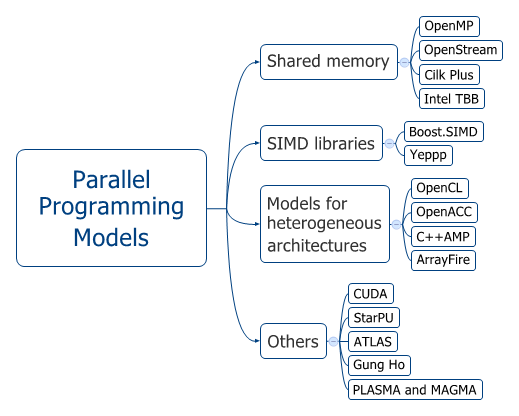
\includegraphics[width=4in]{img/overview}}
\caption{Parallel programming models overview diagram.}
\label{f:overview}
\end{center}
\end{figure}

\subsection{Shared memory}

Multithreading approaches exploit \gls{shared memory} architectures by optimally distributing the workload to different execution units called \glspl{thread}. A program creates threads when performing parallelism, which are sequences of instructions, and the system scheduler is responsible for assigning threads to the physical cores of the device where the program will run (usually with some user direction involved).

Depending on the platform and the programming language used, thread affinity controls may be used to map specific threads to specific cores, making the scheduling process deterministic and giving the programmer better control to exploit and measure parallel performance.

Knowledge of shared memory architectures and their performance considerations yields better results when writing multithreaded programs, as optimum performance is dependant on many factors related to the memory hierarchy~\cite{dagum1998openmp}. Multithreading has been associated with bugs because of this, since dealing with concurrency and synchronisation problems adds a layer of complexity to any program written with multithreading in mind.

However, many languages and libraries have been created to minimise these disadvantages and multithreading has become a simpler activity. Key developments are described next.

\subsubsection{OpenMP}

Open Multi-Processing (OpenMP)~\cite{dagum1998openmp} is both a library and an extension to Fortran, C and C++ for writing parallel, thread-based programs for shared memory architectures, and supports accelerators as of version 4.0\cite{openmp13}. Originally designed for exploiting data parallelism over loops, task parallelism support was added later in version 3.0~\cite{tousimojarad2014comparison}.

The OpenMP standard was created in 1997 by \textit{OpenMP Architecture Rating Board}, a consortium conformed of hardware and software vendors like Intel, AMD, Cray, IBM, HP, Nvidia, Texas Instruments, Red Hat, Oracle, etc. It supports popular Unix-like and Windows platforms.

OpenMP has been popular for scientific HPC because it is possible to modify an existing Fortran or C/C++ program to exploit multi-core architectures and it is supported by many compilers~\cite{2_openmp.org_2015}. In comparison with native models such as POSIX threads\cite{mueller1993library}, OpenMP code can be shorter and more robust, without a negative impact on performance and with no changes to the application logic~\cite{kuhn2000openmp}.

\subsubsection{Open Stream}

OpenStream is a streaming programming language~\cite{pop2013openstream}, defined as an extension to OpenMP. It was designed to exploit pipeline parallelism, used to exploit parallel architectures processing streams of data. It functions as another tool to create parallel algorithms which behave differently from data or task parallelism. It is available as a custom version of GCC, which needs to be built from source.

While there are no references in the literature of using OpenStream with a Xeon Phi accelerator, it would be possible because the Xeon Phi is a shared memory architecture. Further experiments would be needed to know if speedup is feasible, since both vectorisation and cache locality are vital to maximise the performance of the Xeon Phi accelerator\cite{7_software.intel.com_2014}.

\subsubsection{Cilk Plus}

Cilk Plus~\cite{robison2012parallel} is a programming language launched by Intel in 2009, defined by the same rules and semantics of the C/C++ languages, with extensions for parallel computing (in a similar fashion to OpenMP). It resulted as a combination of previous work done for the Cilk and Cilk++ languages.

As a successor to Cilk~\cite{frigo1998implementation}, created in 1994, it shares the idea of a runtime providing task parallelism with a sophisticated dynamic scheduler using work stealing, along with an interface to exploit it by using the new ``spawn'' and ``sync'' keywords. The programmer writes code with these keywords, expressing that there exist opportunities for parallelism in certain parts of the code. The runtime will determine if it is efficient to execute those sections in parallel. Special profiling and debugging tools by Intel exist to understand how the runtime is affecting programs and understand the utilisation of the hardware~\cite{1_cilkplus_2015}.

Cilk Plus also adds support for parallel for-loops and a special array notation that can exploit SIMD for data parallelism. The array notation has support for slices, as seen in higher-level languages like Python~\cite{2_wikipedia_2015}. Basic vector operations like sums, multiplications and copies can be expressed with standard operators~\cite{3_cilkplus_2012}. These two features, along with new keywords for vectorisation hints to the compiler, remove responsibility from the programmer and delegate it to the Cilk compiler and runtime.

Compiler support for Cilk Plus is not as ample as OpenMP's, but Intel has provided support for GCC, LLVM/clang and the Intel C++ Compiler~\cite{3_wikipedia_2015}.

\subsubsection{Intel TBB}

Intel Threading Building Blocks (Intel TBB) is a C++ library that provides concurrent data structures, parallel algorithms and high-level routines for multithreading programs~\cite{tousimojarad2014comparison}. As a stand-alone library, it requires no additional compiler support and may be included in existing C++ programs, though some functionality may only be restricted to the processor model used and its capabilities.

In order to incur as little overhead as possible, a lot of of the code is processed at compile time using the C++ template mechanism, thus providing efficient, low-overhead polymorphism during runtime for its concurrent collections.

Other components for parallel programming include special memory allocation routines for dealing concurrency and false sharing, parallel looping and sorting, wrappers to synchronisation mechanisms and atomic instructions, and skeletons for writing more complex task parallelism.

The ``Flow Graph'' routines also provide an abstraction for task parallelism using message passing between computing nodes, which may be used for \gls{distributed computing}~\cite{robison2012parallel} using MIMD architectures. It is an interface for specifying data dependencies and algorithms to execute in a program as a graph, so it can be naturally mapped to a distributed system.

Another feature is a ``speculative locking'' mechanism introduces to Intel TBB, which can take advantage of a processor's support for  Transactional Synchronization Extensions instructions~\cite{yoo2013performance}. This may be an opportunity to achieve performance in critical pieces of code with a low level of concurrency.

Lastly, other C++ libraries can use Intel TBB features for their own purposes. AMD's open source Bolt C++ library~\cite{10_amd_2015}, which provides facilities for CPU and GPU computing, optionally uses Intel TBB as a back-end for CPU parallel computing, in the event that a GPU was not found.


%\subsection{Message passing}

%\subsubsection{MPI}

%The Message Passing Interface (MPI) is a library with a standard specification for writing parallel programs using the message-passing model. *** More stuff coming.

%\subsubsection{Hadoop}

\subsection{SIMD libraries}

When dealing with array-based algorithms and operations, using the \gls{vectorisation} capabilities of current processors results in considerable speedup with relatively low effort (compared with multithreading) since many operations can be executed at the same time by using SIMD assembly-level instructions. Hardware vendors have supported the continuous development of these instructions for their newer CPU architectures~\cite{lomont2011introduction}~\cite{4_arm.com_2015}.

\subsubsection{Boost.SIMD}

A proposed addition to the popular Boost libraries for C++, Boost.SIMD~\cite{esterie2014boost} provides portable constructs to access SIMD processor instructions and exploit data parallelism. It works by abstracting a ``pack'' of primitive types and subsequent operations to it. As the pack is of a defined width, SIMD operations may be performed in parallel by the processor. It supports multiple CPU architectures and MIC accelerators~\cite{1_numscale.com_2014}.

\subsubsection{Yeppp}

The open source Yeppp library~\cite{4_yeppp.info_2015}, written using the PeachPy~\cite{dukhan2013peachpy} framework, provides specific SIMD versions of vector-processing functions (primitive operations like sums, multiplications, dot products, trigonometry, etc.) for CPU-based architectures, including the Xeon Phi accelerator. The functions are written as low-level assembly embedded in Python code, which is maintained and tuned for different CPUs and MIC accelerators. While the instructions are written using assembly languages, a Python interpreter can provide additional functionality for profiling and debugging code, as well as access to its standard library, making the creation of low-level programs more accessible.

The Yeppp library has very specific functions, they can be used as building blocks for building more complex HPC applications efficiently, provided data dependencies are suitable and cache sizes are taken into account.

It is similar in spirit to the commercial Intel Integrated Performance Primitives (Intel IPP)~\cite{5_software.intel.com_2015}, which is another collection of optimised vector-processing functions (albeit a more complete offer, with digital signal, image and speech processing functions, which can also make use of OpenMP internally to exploit multithreading and SIMD instructions at the same time). Intel IPP supports mainly Intel processors (and Xeon Phi accelerators) and their SIMD instructions, but Yeppp is designed to exploit SIMD instructions for x86 (Intel and AMD), ARM and MIPS processors. There exist official bindings for C, C++, Fortran, Java and C\#, while Intel IPP only has official bindings for C, but there are third party bindings for Python, Ruby and C\#, as well as support for calling the functions from Java.



\subsection{Models for heterogeneous architectures}

Models compatible with different kinds of architectures share the idea of mapping input and output data to the particular cores of the parallel hardware, either implicitly or explicitly. Implicitly mapped approaches are simpler to program with, but might not offer as much flexibility when tuning code for particular performance needs. In contrast, explicit mapping of data to cores requires more low-level knowledge of the underlying hardware (especially of the memory model) but provides greater flexibility.

\subsubsection{OpenCL}

The Open Computing Language (OpenCL) framework~\cite{stone2010opencl} provides a single interface to write kernels that can be executed in many kinds of processors and accelerators, like CPUs, GPUs, APUs, Xeon Phi, FPGAs and Digital Signal Processors. It provides execution, synchronisation and memory models for data parallelism. The standard was created by Apple in collaboration with AMD, Intel, Qualcomm, Nvidia and IBM. A proposal for an open standard was submitted to the Khronos Group (a consortium created by members from Apple, IBM, Intel, AMD, Altera, Nvidia and others~\cite{6_wikipedia_2015}, involved in overseeing the creation of other open standards like OpenGL, SPIR and Vulkan)~\cite{11_khronos.org_2015}, who released version 1.0 of the new OpenCL standard in 2008.

OpenCL provides a low level interface to different hardware devices capable of performing computations. Based on C, it places the responsibility of handling memory and understanding the way each hardware piece works to the programmer. This makes it both powerful and complex in comparison to other approaches. 

Since hardware evolves quickly and devices have different technical specifications, performance portability is not guaranteed and an OpenCL program is usually designed to exploit the parallel capabilities of a particular kind of processing device (e.g. GPUs) or a particular model of such devices.

Hardware vendors have been supporting it in their products and the specification is maturing. There exist software development kits from Nvidia, AMD, Altera, Xilinx, Intel, ARM and other vendors~\cite{tsuchiyama2010opencl}~\cite{6_wikipedia_2015}~\cite{tsuchiyama2010opencl}~\cite{singh2011implementing}. It is used both as a complete solution and as an intermediate language for other languages or models, as described in other approaches in this section.

OpenCL abstracts many concepts that can be mapped into different architectures, and provides a framework for manipulating these concepts and building programs that can then be executed in very different architectures. One important part of the OpenCL paradigm is the execution model, described in detail in~\cite{khronos44opencl}. It differentiates between \textit{host programs} (written in C, C++ or any other language with a binding to OpenCL, and compiled by the host) and \textit{kernels} (written in OpenCL C and compiled on the device). In a host program, a context and a command queue are created, with which commands can be issued from the host to the device (Figure~\ref{f:enqueue}). Commands include memory transfers, memory partitioning, kernel executions and synchronisation.

\begin{figure}[!h]
\begin{center}
\centerline{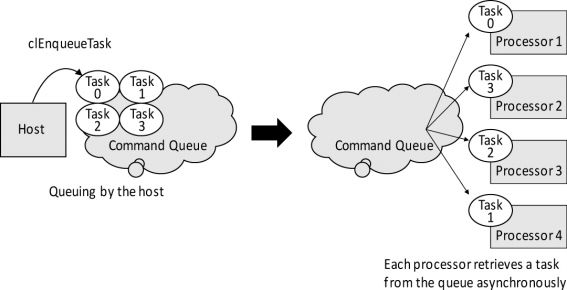
\includegraphics{img/enqueue}}
\caption[OpenCL Command queues as issued by the host and carried out by the devices.]{OpenCL Command queues as issued by the host and carried out by the devices~\cite{tsuchiyama2010opencl}.}
\label{f:enqueue}
\end{center}
\end{figure}

When the host program schedules a kernel execution, one or more \textit{\glspl{work-item}} are created and each execute the kernel once. Work-items are mapped into a n-dimensional range index space, called \textit{\gls{NDRange}}. This index space dictates how many work-items are created, i.e. the \textit{\gls{global work size}} of the command. Each work-item is issued a global ID number according to its position in the NDRange. With this ID number, work-items may be mapped to different sections of input and output data. 

Work-items are then organised in \textit{\glspl{work-group}}, which are mapped to the NDRange. The size of the dimensions of each work-group can be specified, which will determine the number of work-groups to create, i.e. the \textit{\gls{local work size}}. Figure~\ref{f:work2d} illustrates a simplistic example using two dimensions.

\begin{figure}[!h]
\begin{center}
\centerline{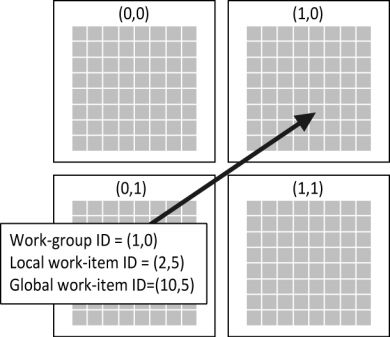
\includegraphics{img/work2d}}
\caption[Example of an OpenCL 2D-NDRange and its ID numbering.]{Example of an OpenCL 2D-NDRange and its ID numbering~\cite{tsuchiyama2010opencl}.}
\label{f:work2d}
\end{center}
\end{figure}

Each created work-group is mapped to a specific ``compute unit'', a concept that varies depending on the device. Just as each work-group is N-dimensional, each compute unit is also composed of one or more ``\glspl{processing element}'' (or PEs), which are the hardware resources that execute the actual kernels. Figure~\ref{f:hostdev} shows the relationship between these concepts.

\begin{figure}[!h]
\begin{center}
\centerline{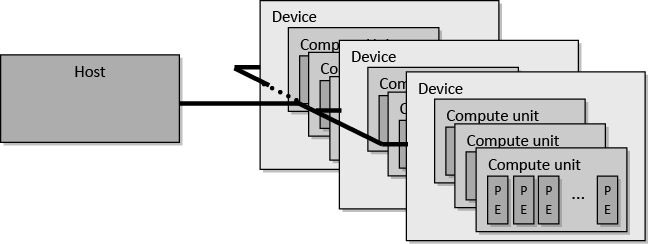
\includegraphics[width=4in]{img/hostdev}}
\caption[OpenCL host and device abstraction.]{OpenCL host and device abstraction~\cite{gaster2012heterogeneous}. A ``PE'' refers to a Processing Element. A single host may access and issue commands to many devices.}
\label{f:hostdev}
\end{center}
\end{figure}

Some concepts can be mapped directly to concepts appearing in the CUDA programming language (surveyed later in this chapter), e.g. OpenCL hosts are similar to OpenCL devices, OpenCL work-items are similar to CUDA threads, and OpenCL work-groups are similar to CUDA thread blocks~\cite{7_amd_2011}. Furthermore, the memory model is similar and the synchronisation guarantees are the same, etc~\cite{7_amd_2011}. Nevertheless, some effort of rewriting significant portions of code is still needed when porting between CUDA and OpenCL. There are no performance differences between these two languages when code is written carefully~\cite{fang2011comprehensive}.

%*** Different things from CUDA... 
%AMD COMPATIBLE

Because OpenCL is compatible with many devices, achieving good performance requires knowledge of the underlying hardware, as well as insights into how an OpenCL implementation interfaces with said hardware. Many low-level details, like memory transfers, are delegated to the programmer~\cite{augonnet2011starpu}. Each vendor usually publishes programming guides and articles for their specific devices, e.g. for Altera for FPGAs~\cite{singh2011implementing}, or Intel for the Xeon Phi~\cite{7_software.intel.com_2014}. Thus, there are many considerations to take into account when programming HPC with OpenCL, regardless of the device.

%*** Stuff about Xeon Phi

The most recent version of the OpenCL standard, version 2.1 released in 2015, adds support for some C++ features. OpenCL has third party bindings for Java, Python, the .NET platform languages and Javascript. The Javascript binding, the WebCL standard~\cite{aarnio2014webcl}, is of special interest since it will allow web applications to exploit parallel architectures on the client-side, extending the range of applications that might become available to users inside a web browser~\cite{herhut2012parallel}.

\subsubsection{OpenACC}

Open Accelerators (OpenACC)~\cite{Group2013} is language extension for Fotran, C and C++, similar to OpenMP, with a focus on interfacing with accelerators. It was created by Nvidia, Cray, CAPS and PGI, and aims at providing a simple interface to exploit data parallelism on accelerators in existing Fortran, C and C++ programs.

At this time, OpenACC compiler support is poorer than OpenMP's. The GCC compiler has preliminary support for OpenACC 2.0 since version 5.0, but there is no current support for OpenACC in clang, or in the Intel C++ or Fortran Compilers~\cite{4_openacc.org_2015}.

\subsubsection{C++ AMP}

C++ Accelerated Massive Parallelism (C++ AMP) is an extension~\cite{Microsoft2013} to the C++ language to support parallel computing on both CPUs and GPUs, providing constructs for creating algorithms from parallel loops using anonymous functions that map to accelerators. Data distribution among cores (whether they are CPU or GPU cores) is done automatically. It was created by Microsoft in 2012.

Users can specify which accelerator to use \textit{a priori}. If no accelerator is specified C++ AMP will choose a suitable one provided it can detect it. If no accelerator was detected, it will fall back to use the host CPU (in a multi-core fashion if supported) and use SIMD instructions instead, if supported by the processor.

While historically available for Microsoft technology stack (Visual C++ and Direct3D), there exist two clang/LLVM implementations, one effort by Intel~\cite{Sharlet2012} and another open source effort by AMD~\cite{8_blogs.msdn.com_2015}~\cite{9_bitbucket.org_2015} that compiles code to OpenCL, providing cross-platform usability and support for a wider range of GPUs and AMD APUs. The AMD implementation also has support for the newer SPIR intermediate language (previously mentioned in the OpenCL section).

There is currently no information regarding support for MIC accelerators, limiting its use in pursuing performance portability. Since the clang/LLVM version compiles to OpenCL, supporting this and other accelerators is theoretically sound.

\subsubsection{ArrayFire}

ArrayFire~\cite{malcolm2012arrayfire} is a C++ library that provides several routines for data parallelism in CPUs, GPUs, APUs and MIC accelerators, with no extra support needed from a compiler. Originally a commercial offering from AccelerEyes, it was released as an open source project in late 2014~\cite{5_arrayfire_2014}.

ArrayFire approaches the portable performance problem directly, supporting as many different devices and tuning its library functions for optimum performance. It offers binary installers, but the library may be built from source for different platforms by selecting which components and kernel versions will be compiled (e.g. it will not compile CUDA versions of the kernels if there is not a CUDA SDK present).

The ArrayFire \glspl{kernel} are implemented in CUDA, OpenCL and C++ to support many devices. C++ template meta-programming techniques and a Just-In-Time compilation approach provide fusing of kernels to minimise synchronisation and communication overheads.


\subsection{Others}

Programming models not fitting into one of the previously defined categories will be described next. This other interesting lines of research in the same vein are frameworks like StarPU~\cite{augonnet2011starpu}, auto-tuning optimisation approaches like the ATLAS library~\cite{whaley2001automated}, machine learning methods~\cite{ganapathi2009case} and parallel compilers like the Gung Ho project~\cite{ford2013}.

\subsubsection{CUDA}

The Compute Unified Device Architecture (CUDA) platform~\cite{3_nvidia.com_2015} provides a programming language based on C to write programs that exploit data parallelism on GPU accelerators made by Nvidia in 2007. It was one of the first platforms to give a general purpose interface to developers without the need to interface or have knowledge of the original purpose of the GPU hardware, i.e. graphics processing.

It still requires the programmer to learn the specific execution, synchronisation and memory models provided by CUDA and to understand the technical specifications of the accelerator in detail. The programming model itself deals with memory hierarchy and patters for efficient memory access. It does not guarantee performance portability as models of Nvidia GPUs differ with every new generation~\cite{6_developer.nvidia.com_2015}.

%Designed for data parallelism, it is not immediately useful for \gls{task parallelism} (((or fine-grained parallelism? a reference is needed here))).

The CUDA platform is reviewed in this section because of its similarity with OpenCL and its historical niche on the creation of new parallel programming models. It has influenced other programming models like OpenCL (surveyed in this section) and can serve as an intermediate language for other, more complex parallel computing approaches~\cite{malcolm2012arrayfire}~\cite{enmyren2010skepu}.

There is overlapping functionality between CUDA and OpenCL, since both may be used to create programs for GPU accelerators and because of the similarity of their programming models. However, there have not been found significant differences between their performance~\cite{fang2011comprehensive}.

The CUDA development tools provided by Nvidia are available for different operating systems. The CUDA C/C++ compiler is written over the LLVM compiler infrastructure. There exists an official Fortran version of the language that integrates the CUDA syntax as a Fortran extension. The compiler for this language is provided by the PGI Group. There also exist third party bindings to many languages, like Java, Python, Perl, Ruby, R, Lua, Haskell, Mathematica, MATLAB and the .NET platform languages~\cite{5_wikipedia_2015}.

\subsubsection{StarPU}

The StarPU platform~\cite{augonnet2011starpu} delivers a framework for writing programs that can be executed on heterogeneous architectures. It provides a runtime capable of scheduling user-defined tasks on different pieces of hardware, by using the native libraries for copying data from the processor to the accelerators and scheduling routines to be executed in those accelerators. StarPU exposes a library that abstracts these different native libraries for scheduling, and that is also capable of using different pre-defined or custom-defined scheduling configurations (i.e. greedy or balanced approaches w.r.t. the size of the tasks to execute).

The StarPU project makes an effort to solve the problem presented in this Dissertation, supporting heterogeneous computing on many different processors and accelerators, including CPUs, Cell, GPUs and MICs. It is able to schedule tasks and express dependencies between them, providing a framework to exploit the performance of multiple processors and accelerators. It also has message-passing capabilities to exploit many multi-core processors and/or accelerators at the same time.

\subsubsection{ATLAS, PLASMA and MAGMA}

Basic Linear Algebra Subprograms (BLAS) is a specification for a low-level, high-performance linear algebra functions and routines~\cite{15_wikipedia_2015}, over which many different applications and libraries have been created, e.g. LAPACK~\cite{anderson1990lapack}. The multiple applications of the BLAS specification makes it a popular target for research in efficient implementations, which also spans research in very different methods of obtaining performance from distinct types of architectures. Popular implementations include the Intel MKL, AMD's ACML, cuBLAS, clBLAS and OpenBLAS~\cite{15_wikipedia_2015}.

Other key projects that potentially could target heterogeneous architectures comprise the ATLAS, MAGMA and PLASMA projects. The Automatically Tuned Linear Algebra Software (ATLAS) project makes it possible to create customised versions of BLAS libraries for a particular architecture automatically~\cite{whaley2001automated}. Generating the implementation may take up to hours because of the necessary search for the optimal configuration, which will strive to optimise cache utilisation and other performance factors. While it currently supports CPU-based optimisations, the optimisation idea feels general enough so that it might be used for heterogeneous architectures in the future.

The MAGMA and PLASMA libraries implement BLAS and a part of LAPACK in a different manner. PLASMA is compatible with CPU-based architectures and focuses on performance on high numbers of cores by allowing fine-grained parallelism on different stage of the functions~\cite{agullo2009numerical}. MAGMA is capable of offloading the computations to different kinds of accelerators, like GPUs~\cite{agullo2009numerical} and MICs~\cite{dongarra2013portable}. It exploits the higher parallelism of these accelerators and minimises their higher memory latency costs (as described earlier in this chapter).

The MAGMA and PLASMA projects achieve performance for heterogeneous architectures by directly coding different routines and maximising their performance for specific hardware. Since BLAS and LAPACK serve as building blocks for different kinds of applications, aiming to provide high-performance implementations of these routines that feature performance portability is a relevant effort.

\subsubsection{Gung Ho project}

Gung Ho is an on-going project by the University of Manchester, the Imperial College London and other institutions, in collaboration with the Met Office and the National Environment Research Council (NERC)~\cite{ford2013}. The premise involves separating the work of writing and executing parallel algorithms among different layers. There are modules for the hardware infrastructure, as well as a driver module that controls the execution of the parallel algorithms, which are encapsulated in ``models''.

A model consists of three different layers. The highest-level layer contains the application-domain algorithms that are written by the programmer, with no required knowledge of the hardware details or the parallelisation of the code. The lowest-level layer contains the kernels that execute the numerical routines and achieve the results expected from the algorithm layer.

The parallelisation occurs in the middle-layer, called the PSy layer. It maps the algorithms written in the high-level layer to the kernels in the low-level layer. It interfaces with the hardware infrastructure to choose the best-performing kernels that can execute the algorithms written, in accordance with the current hardware and using a suitable (and available) parallel programming model, e.g. OpenMP or OpenACC. This interactions between layers appear in Figure~\ref{f:gung}.

\begin{figure}[!h]
\begin{center}
\centerline{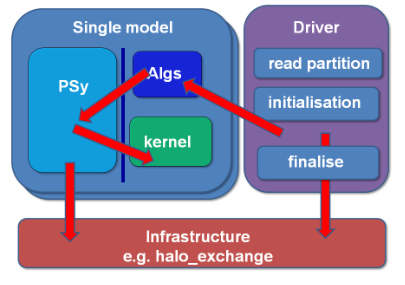
\includegraphics[width=4in]{img/gung}}
\caption[The Gung Ho project approach to abstracting parallelism.]{The Gung Ho project approach to abstracting parallelism, where the arrows show the direction in which data and control flows between connected layers~\cite{ford2013}.}
\label{f:gung}
\end{center}
\end{figure}

There is recent work in automatically generating the code in the PSy layer. The PSyclone module is a parallel compiler for this layer, able to map the algorithm and kernel layers with some added optimisations~\cite{9_puma.nerc.ac.uk_2015}.

The Gung Ho project serves as an original inspiration for this currently presented Dissertation. Other Dissertation projects in the Advanced Processor Technologies group of the University of Manchester work directly on it. As reference, a similar ideology for abstracting parallelism may be found in~\cite{Kelly}.

% TODO uo!?

%\subsubsection{Unified Parallel C}

%Some stuff.

\subsubsection{Machine learning methods}



\section{The case for performance portability}

\subsection{Why heterogeneous architectures?}

*** Different hardware is good for different things, multi-core scaling in different devices and reaffirm the importance of parallelism, expose other research areas like big.LITTLE ***

~\cite{daga2011efficacy}
~\cite{zhu2013high}
~\cite{AMD2011}

\subsection{Classification of programming models}

In this section, a classification of the programming models and languages surveyed is proposed, along with their summarised characteristics in terms of performance portability. Table~\ref{t:portability} shows this classification.

\begin{table}[!h]
\begin{center}
\centerline{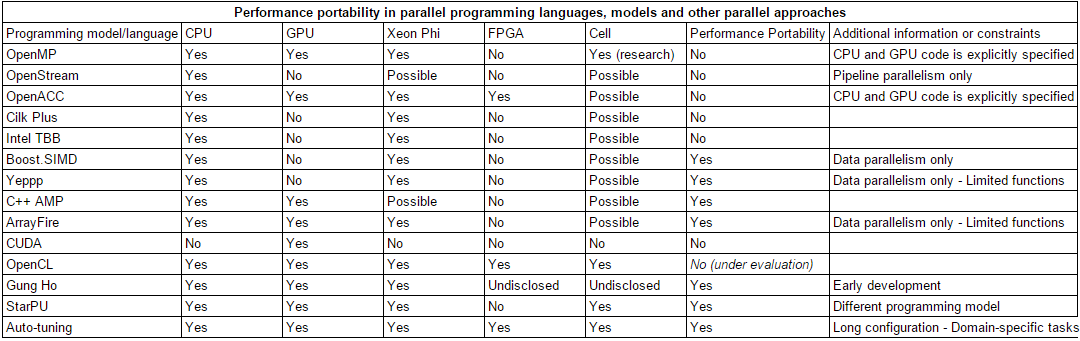
\includegraphics[width=\columnwidth]{img/portability}}
\caption{Performance portability in parallel programming languages, models and other parallel approaches.}
\label{t:portability}
\end{center}
\end{table}

Thinking about hardware, many types of parallel hardware are bound to be mixed together to create heterogeneous systems. Other hardware choices like the Cell processor have not been popular, which means that programs specifically tuned to exploit their performance, along with platform-specific programming models or languages, may become obsolete in the future and extra work will be necessary to port these efforts to more suitable platforms.

From the hardware described, in relation with the compatibility of the programming models. Give the popularity of GPU accelerators, specially on mobile devices, it is important blah blah
2
The production of new programming languages and models, specially those that are able to exploit parallelism, % TODO explain why it might be complex!

OpenCL solved the code portability problem that existed between different types of architectures. While this was a step forward, the portability of performance is an important feature to pursue in a programming model, given the variety of heterogeneous architectures.

\section{Summary}

The information presented in this chapter is useful to understand why performance portability is a subject worth researching. The wide variety of parallel architectures, parallel hardware and their programming models and languages means extra effort for programmers interested in HPC. Some approaches that already deal with performance portability for heterogeneous architectures have been explained and will be evaluated in the remainder of this Dissertation, as discussed in the next chapter.

\chapter{Research methodology}
\label{cha:methodology}

This chapter presents the research methodology on which the project will be based. In Section 3.1, the reference paper that the project initially seeks to reproduce will be discussed. In Section 3.2, the parallel hardware platforms that are available for experimentation will be described, along with the programming languages and models that they can support. In Section 3.3, the algorithm selected as a means of demonstrating parallelism on the target architectures will be described, with references to its origin and available implementations (both serial and parallel) from previous work. Section 3.6 discusses which of the programming models and languages reviewed in Chapter 2 are available for use in the hardware available for experimentation. In Section 3.5, the evaluation criteria for measuring the results obtained during the experiments performed as part of the project will be discussed.

\section{Approach to Portable Performance}

As mentioned during the introduction, performance portability will be attempted, based on the work done in~\cite{dolbeau2013one}. As mentioned in the previous chapter, the OpenCL framework offers suitable abstractions to create programs for a wide range of parallel architectures, but performance portability is not guaranteed.

The main experiment of the project will consist in understanding how the execution model configuration (NDRange, global and local work sizes, as described during Chapter 2) of a particular program may be tuned for different purposes, e.g. obtaining optimal performance for one particular architecture. This parameters may be configured globally in a program, so that all executed commands share the same configuration, or it may defined independently for each command to execute~\cite{khronos44opencl}.

Choosing a global work size is an easy task because, as explained in Chapter~\ref{cha:back}, it maps directly to the calculations that the algorithm must perform. The same situation happens with the NDRange details, because the number of dimensions that will be used is also problem-dependant, as different dimensions map better (or worse) to different kinds of problems.

The choice of a local work size has been identified as a more important factor for performance~\cite{Rosenberg2011}. In particular, it has been proposed that the local work size of a program can be tuned to get good performance from heterogeneous parallel architectures~\cite{dolbeau2013one}.

When left unspecified, OpenCL automatically selects a default local work size configuration that strives to~\cite{khronos44opencl}. This configuration is implementation-dependant and may only be known until runtime, either by using vendor tools like Intel's vTune~\cite{7_software.intel.com_2013}, or by using the \texttt{get\_local\_size} function defined by the OpenCL standard. It may not be the case that this default configuration is the optimal.

Manually choosing an adequate local work size is not a simple task, as there are many factors to consider. It is not always the case that choosing bigger or smaller local work sizes results in better performance, but because of the particularities of each OpenCL implementation and the technical specifications of each hardware device, there is not a defined methodology for finding an optimal size other than doing several experiments with different configurations~\cite{Rosenberg2011}~\cite{dolbeau2013one}.

Usually, this parameter is tuned for optimal performance on a particular model of parallel hardware. In this manner, specific versions of code are produced for every kind of architecture, and for particular models. Just as the CUDA model discussed in the previous chapter, which targets Nvidia GPUs only, performance portability is not guaranteed even when programming for the same type of architecture as the specifications of every new model may be very different.

By selecting an appropriate local work size, performance losses across all targets can be minimised and good parallel performance can still be obtained from different parallel architectures~\cite{dolbeau2013one}.

\section{Available hardware}

There are different architectures available on which to run experiments. While the following sections describe the details of these architectures, technical information has been summarised in Table~\ref{t:hwsum}. As mentioned during Chapter~\ref{cha:back}, it is important to cover modern and popular architectures. This project will perform experiments in CPU-based architectures (both multi-socket configurations and MIC devices), as well as GPU accelerators.

\begin{table}[!ht]
\begin{center}
\centerline{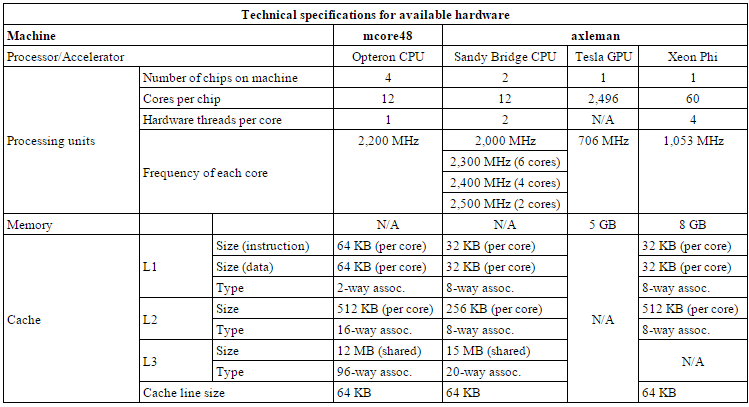
\includegraphics[width=\columnwidth]{img/hwsum}}
\caption[Summary of technical specifications of available hardware.]{Summary of technical specifications of available hardware, including main processors and accelerators. Configurations and frequencies of cores may be seen, along with details of the memory hierarchy of each chip.}
\label{t:hwsum}
\end{center}
\end{table}

%, 

\subsection{mcore48}

The mcore48 is a Dell machine composed of a four-chip board containing AMD Opteron 6174~\cite{amd} chips with 12 cores clocked at 2200 MHz. This CPU is based on the K10 microarchitecture. The L1 cache level has a Least Recently Used (LRU) replacement policy and a write-allocate policy, while both L2 and L3 cache levels have a pseudo LRU replacement policy. L3 cache level is shared, connected to all cores by a 3200 MHz HyperTransport bus.

The mcore48 has no addtional accelerators installed. The operating system running on the mcore48 is CentOS, version 6.5.

\subsection{axleman}

The axleman machine is more versatile than the mcore48. While in terms of CPUs it has a lower number of cores with lower frequencies and cache capacities, the CPUs in axleman have certain differences versus the CPUs on mcore48, as will be described in the following sections. It also comes equipped with two kinds of accelerators, making it a very important piece of hardware for the experiments that will be done during the project.

The operative system running on the axleman is CentOS, version 6.6.

\subsubsection{Sandy Bridge CPU}

Axleman is installed with two Intel Xeon E5-2620 x86-64 CPUs connected with Intel's QuickPath Interconnect (QPI) clocked at 3600 MHz, providing a point-to-point processor interconnect between these CPUs. This enables Non-Uniform Memory Access (NUMA). Programs may access data from both CPUs without any additional specifications and the programmer can think of the two processors as one big processor, even if memory accesses from one core to another have different access times (hence the NUMA classification).

The Xeon E5-2600 family of processors is based on the Sandy Bridge microarchitecture, released in 2011. It targets a 32 nanometer fabrication process. A single E5-2620 has six cores clocked at 2 GHz base frequency and at 2.5 GHz Turbo Boost frequency (depending on the number of cores working). It has support for HyperThreading (Intel's version of simultaneous multithreading), for a total of 12 hardware threads available~\cite{1_cpu-world.com_2015}. Cache sizes can be seen in Table~\ref{t:hwsum}.

This particular configuration of two CPUs installed on axleman will be referred to as the ``Sandy Bridge CPU" in the remainder of this document.

\subsubsection{Kepler GPU}

Axleman has additional accelerators installed. One of them is a Nvidia Tesla K20m GPU~\cite{6_gpuzoo.com_2015}, which has 2,496 cores and 5 GB of ram on-chip, organised in 20 blocks of 64M x 16 GDDR5~\cite{Nvidia2013}. The K20m is based on the Kepler GK110GL microarchitecture~\cite{Nvidia2012}. Details about the memory hierarchy can be seen in Table~\ref{t:hwsum}, though it works differently than that of CPU-based architectures. The Kepler GPU is connected to axleman with a PCIe x16 bus.

\subsubsection{Xeon Phi}

Axleman also has a MIC accelerator. The Xeon Phi model installed is the 5110P~\cite{3_cpu-world.com_2015}, with 60 cores, and uses a 22 nanometer fabrication process. Each core is a simple 64-bit Pentium processor, with an x86 ISA, clocked at 1,053 MHz. Each core also has a VPU capable of performing FMA operations with 512-bit SIMD vector registers. Because of 4-way multithreading, the Xeon Phi has a total of 240 hardware threads available. Cache and memory details may be consulted in Table~\ref{t:hwsum}, as defined in~\cite{5_intel_ark_productspecs_2015} and~\cite{4_software.intel.com_2012}.

The ``Xeon Phi", as the Xeon Phi model 5110P that is installed on axleman will be referred to from this point forward, is connected to axleman by PCIe x16.

\section{Algorithm selection: Shallow water simulation}

An algorithm will be used which is:
\begin{itemize}

\item Performance-relevant (a building block for other algorithms, universally used and actively surveyed in the literature).

\item Capable of demonstrating common bottlenecks in parallel computing.

\item Simple enough to provide reasonable modifications that increase its performance in heterogeneous architectures.

\item Interesting, such that optimisations may be useful for the continuous development of science.

\end{itemize}

Previous work in this domain has used a shallow water simulation as part of climate modelling. It presents opportunities for parallelism which have also been studied on the same (or very similar) hardware that was listed on this chapter, as seen in~\cite{pappas2012} and in~\cite{Cheng2014}.

\subsection{Complexity analysis}

The algorithm presents quadratic space and time complexities.

\begin{table}[!h]
\begin{center}
\centerline{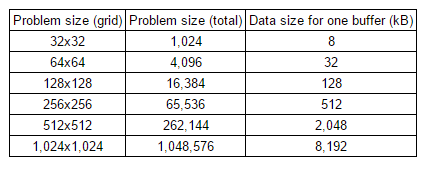
\includegraphics[width=3.5in]{img/problemsizescaling}}
\caption{Shallow water space complexity details.}
\label{t:space}
\end{center}
\end{table}


\begin{figure}[!h]
\begin{center}
\centerline{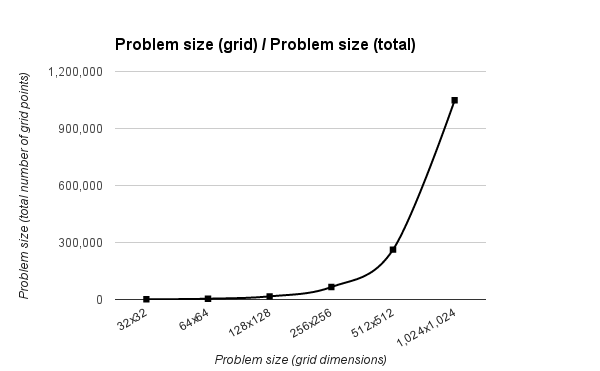
\includegraphics[width=5.5in]{img/problemsizeplot}}
\caption{Shallow water space complexity scalability plot.}
\label{f:spaceplot}
\end{center}
\end{figure}


\subsection{Code versions available from previous work}

The original serial Fortran version of the shallow water simulation used in this project was written by Paul N. Swarztrauber in 1984. The shallow water model is based on previous work from 1975~\cite{sadourny1975dynamics}. The performance of this version, as well as other parallel implementations, was thoroughly studied at the time of its creation~\cite{mcbryan1988new}. A port of this serial version to the C language was provided by Graham Riley (project supervisor) for this project.

There exist OpenMP and OpenCL versions created during the work done in~\cite{pappas2012}. The OpenCL version was specifically tuned for performance on an Nvidia Fermi GPU (a generation older than the currently installed Kepler GPU). As mentioned in Chapter~\ref{cha:back}, OpenCL does not aim for nor guarantee performance portability, so work may be needed to correctly exploit the performance achievable by the hardware currently available.

\section{Programming languages and available compilers}

The main platform in which to evaluate parallel performance will be OpenCL. As mentioned in~\cite{dolbeau2013one}, the OpenCL framework offers the unique opportunity to target different parallel architectures without changes to the code.

The code running on the host which will create the necessary contexts to run the kernels is written in C. The kernels, which are the pieces of code running on the device, are written in OpenCL's own C subset.

The available C/C++, Fortran, OpenCL and additional compilers and their versions for each piece of available hardware previously described can be seen in Table~\ref{t:compilers}. Axleman provides more varied compiler options relevant for the project, including OpenACC (though the current version only has support for Nvidia GPU accelerators, newer versions also support the Xeon Phi), while the Intel Fortran compiler in the mcore48 supports the newest version of OpenMP (which has accelerator support).

\begin{table}[!h]
\begin{center}
\centerline{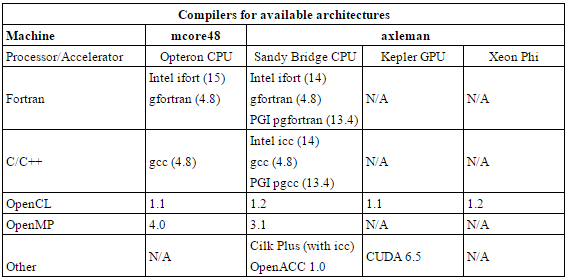
\includegraphics[width=\columnwidth]{img/compilers}}
\caption{Compilers for available architectures.}
\label{t:compilers}
\end{center}
\end{table}

\section{Evaluation}

Execution time ($T$) will be measured from parallel versions of the program running on the different architectures available. Performance will be measured as the inverse of time ($R = \frac{1}{T}$). Speedup will be calculated using Amdalh's Law~\cite{eager1989speedup} against a reference serial version (C, Fortran or OpenCL).

Execution time spent during memory allocations, either in the host or the device, or during memory transfers from the main memory to a device (and viceversa) will not be considered as the interest of the project lies in evaluating floating-point calculation performance. Memory allocations are traditionally complex~\cite{arpaci2012operating} and costly~\cite{detlefs1994memory} and hard to predict in terms of time of execution, mainly because of hardware and operating system performance techniques~\cite{herter2014timing}. Memory transfers, as explained during Chapter~\ref{cha:back}, are slow when considering that the accelerators on axleman are connected to a PCIe bus. Both factors provide additional overheads not directly related to the floating-point performance of the cores that will execute the program and perform the actual calculations.

The current version of the program will also make use of double-precision floating-point numbers. As evaluated in~\cite{pappas2012}, using single-precision variables provides better performance, at least on GPU devices. TODO less precise??? ASK GRAHAM!

Measuring performance using the specific roofline model~\cite{williams2009roofline} for each piece of parallel hardware available is to be considered for this project as well, provided enough time remains after experimentation. The roofline model is able to provide a visual representation of the achieved performance, while referencing directly vendor specifications and extensive benchmarking on a device, measuring performance in floating-point operations per second.

Various problem sizes for the shallow water simulation will be considered in order to better understand parallel hardware behaviour under different memory requirements. These problem size choices, which map directly to the global work size of an OpenCL program, might also affect the possible local work sizes available for experimentation for OpenCL versions of the program.

The OpenCL version will be tuned for specific architectures, varying the work-group dimensions as explained in this chapter. Another tuned version able to obtain reasonable speedup from heterogeneous architectures without changing the code will be sought. The initial search space of work-group dimensions configurations to experiment with is the same considered in~\cite{dolbeau2013one}, also listed in Table~\ref{t:wg}, but more fine-grained configurations may also be attempted.

\begin{table}[!h]
\begin{center}
\centerline{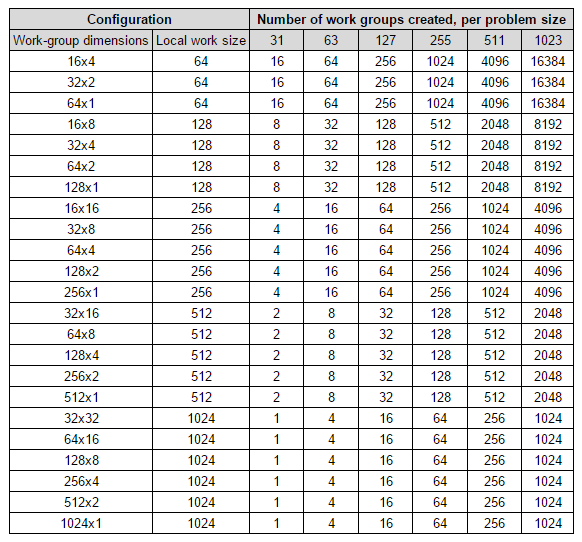
\includegraphics[width=5in]{img/wg}}
\caption{Work-group dimensions configurations for initial experimentation.}
\label{t:wg}
\end{center}
\end{table}

\begin{figure}[!h]
\begin{center}
\centerline{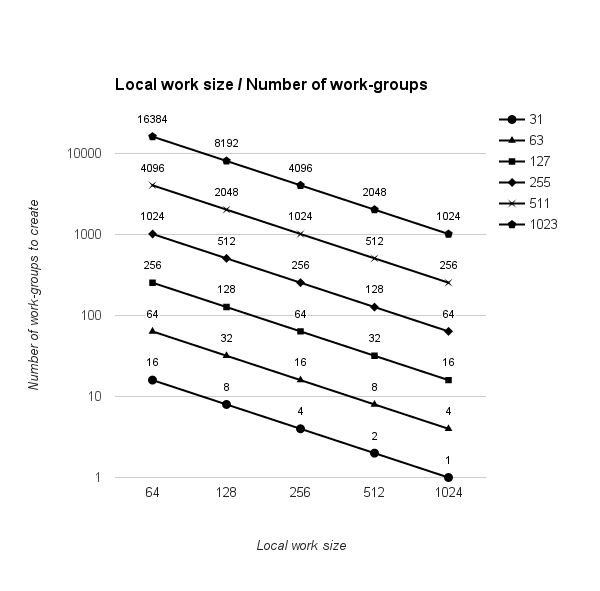
\includegraphics[width=5.2in]{img/wgplot}}
\caption{Work-group dimensions configurations for initial experimentation.}
\label{f:wgplot}
\end{center}
\end{figure}

The project will also seek to improve the performance of the current OpenCL version running on the Xeon Phi accelerator following the methodology of~\cite{7_software.intel.com_2014}, since the current version is not optimal~\cite{Cheng2014}~\cite{7_farber_2012}. For this, an attempt to understand the performance of this version in terms of its overheads will be made, though the inherent difficulty of tuning for performance is to be considered a priori~\cite{riley1997performance}.

% TODO The production of a new version in another programming language that can better exploit parallelism from this accelerator might also be considered.

Because of many different factors, execution time of repetitions of computational experiments tend to differ from one another, even under the same experimental conditions, sometimes significantly~\cite{nogueira2014experimental}. For this reason, the results obtained during the project will be evaluated to be statistically significant by measuring the square-mean error of 10 repetitions of executions under the same experimental conditions.

\section{Summary}

In this chapter, research and evaluation methodology for this project has been explained. The reference literature on which the project is based has been discussed in detail, with analysis in the context of the hardware available for experimentation and the programming models and languages which are supported by it. It is important to consider all previous work done in parallel implementations of shallow water simulations in order to advance research in performance portability, while maintaining a scientific approach to evaluate the results obtained.

\chapter{Experimentation}
\label{cha:exp1}

\section{PHI FAST}

\section{Cache data locality}

\section{Optimization, local work size}

\section{Understanding scheduling}

\section{Summary}
\chapter{Experimentation}
\label{cha:exp2}

The current chapter will present the progress that has been achieved during the time devoted to the project. Section 4.1 will state on which experimental conditions work is being performed. Section 4.2 will present performance results of serial and parallel versions of the shallow water simulation as defined in Chapter 3.

It is worth noting that all code developed for the project, along with scripts for repeating executions, obtaining statistics and creating relevant plots, may be found in~\cite{arturo_isai_castro_perpuli_2015_16985}. Previous serial, parallel and experimental versions of the code have also been added as a reference in the same repository.

\section{Conditions of experimentation}

All experiments were conducted with 10 repetitions. A 95\% confidence level is considered in the plots of this project, in accordance with the material and experienced obtained during the COMP60611 course. The reported performance results correspond to the minimum observed time of execution over the 10 repetitions.

All C versions discussed in the results are compiled using the \texttt{-O3} optimisation flag, both on the Intel icc and the GCC compilers.

The problem sizes were chosen to allow proper vectorisation of the code in the OpenCL versions targeting the Xeon Phi processor, specifically. The work sizes must be multiples of 32 for better performance~\cite{Intel2014}. Since the code uses one extra element for padding, then the problem size must be a multiple of 32, minus one element. The actual 

\begin{table}[!ht]
\begin{center}
\centerline{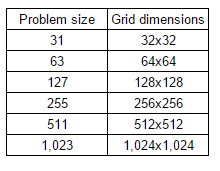
\includegraphics{img/padding}}
\caption[Problem size growth and its effect on the global work size.]{Problem size growth and its effect on the global work size, which denotes the number of work-items to create. The middle column, the total grid size, refers to the size of the actual grid of computational points in the shallow water simulation, including padding.}
\label{t:problemsize}
\end{center}
\end{table}

\section{Results of previous versions}

The previous serial versions (Fortran and C) have been successfully run in the proposed architectures. The compilers used are GCC in the mcore48 (because it is the only C/C++ compiler available for this machine) and Intel icc in the axleman (to link directly with Intel-produced OpenCL libraries on Intel devices). The timing results for the C version obtained in both the mcore48 and the axleman (for CPUs) are in Figure~\ref{f:serial}.

% TODO

\begin{figure}[!h]
\begin{center}
\centerline{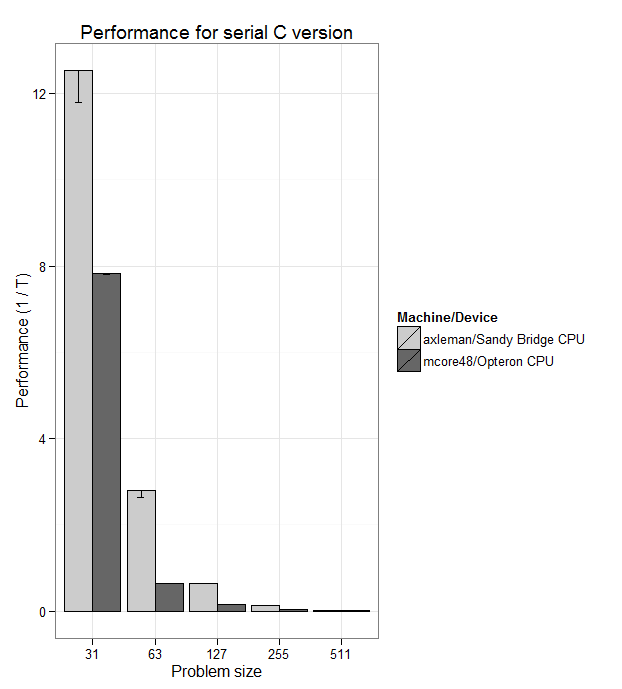
\includegraphics[width=4in]{img/serial}}
\caption{Performance results for serial C version.}
\label{f:serial}
\end{center}
\end{figure}

It can be observed that the Sandy Bridge CPU is faster than the Opteron CPU when using only one core. It may also be noted that performance drops in a non-linear manner when increasing the problem size. While duplicating the problem size means quadrupling the amount of operations that the algorithm will perform,

there are more factors to consider when analysing the scalability of performance on CPUs. Specifically, performance may drop because of the particular characteristics of the hardware used to execute the program.

For instance, one possible cause for additional performance drops in this experiment is the utilisation of slower types of memory (higher levels of cache or RAM) for storing the data of the larger problem. With very small problem sizes, all of the data may fit in the lower, faster levels of cache of a particular CPU used. As the problem size increases, more space is needed for stored data during execution, which may cause cache misses and reduce the performance.

A more comprehensive analysis of the problem sizes, the data needed for the execution of the shallow water simulation, and their relationship with memory types and performance is done in~\cite{pappas2012}. Particular attention is given to the behaviour of performance in multi-core architectures, where other issues like cache coherence and data sharing affect the resulting performance of the algorithm.

\subsection{Results of modifying the local work size}

This section presents the initial experiment of running the code using different configurations of work-group sizes, as shown in~\cite{dolbeau2013one}. The result of this experiment explores the idea that different performance results will be obtained from different work-group sizes, but additional statistical analysis is needed to determine if there is one optimum work-group size that minimises performance losses for all architectures~\cite{dolbeau2013one}.

Work has been directed into understanding the performance of this code when run on the Xeon Phi accelerator to determine whether or not it may be improved upon. The first step was to remove a conditional statement that exists in some of the kernels. As remarked in~\cite{7_software.intel.com_2014}, this branching can prevent the proper vectorisation of the kernels, which is of vital importance to obtaining performance from the Xeon Phi.

As mentioned in the same article, repeatedly calling kernels results in poor performance results when using the Xeon Phi because threads are created with every kernel call. The main loop in the current code calls three different kernels in every iteration. Whether or not this behaviour results in poor performance remains to be proved in this project.

% TODO For the dissertation, a more detailed analysis will be performed using Intel VTune profiler~\cite{7_software.intel.com_2013}.

The OpenCL version has been successfully run in axleman using Sandy Bridge CPU, Tesla GPU and Xeon Phi as different devices, with the same local work sizes as discussed in Chapter 3. The results for the Xeon Phi are in Figure~\ref{f:phi}.

\begin{figure}[!h]
\begin{center}
\centerline{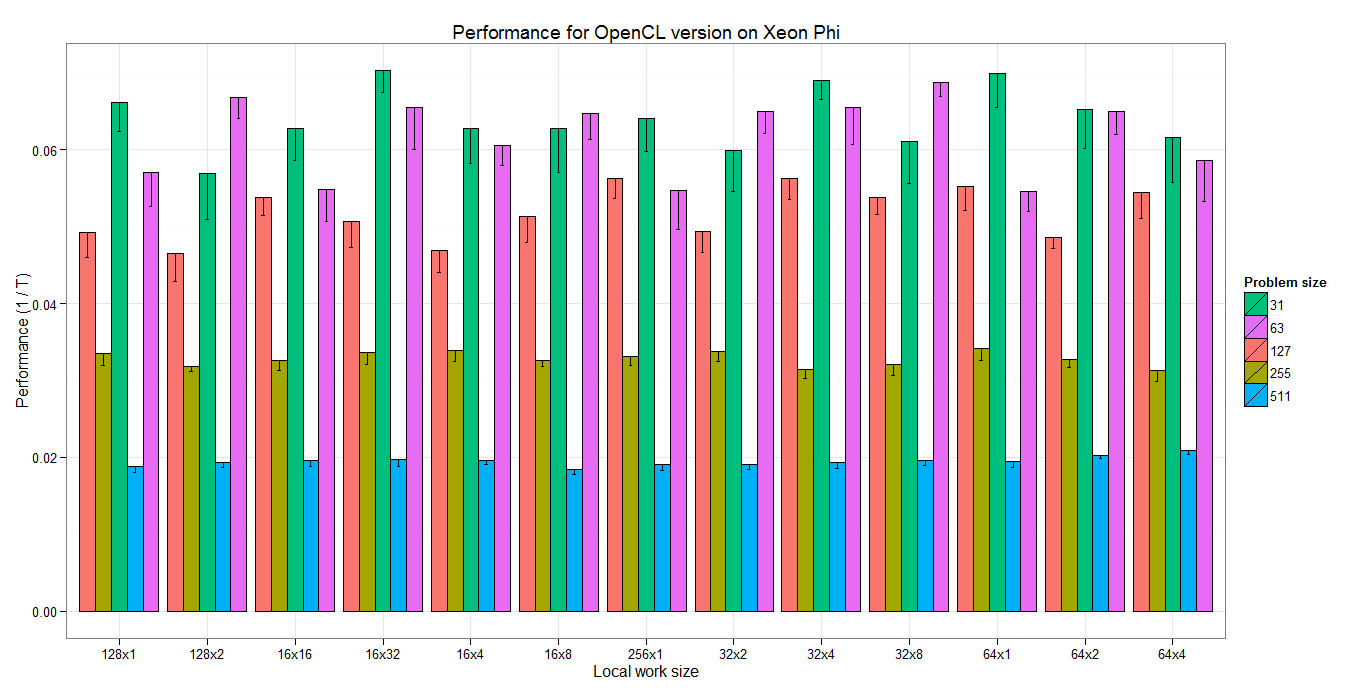
\includegraphics[width=6in]{img/phi}}
\caption{Performance results for OpenCL version running on Xeon Phi.}
\label{f:phi}
\end{center}
\end{figure}

The plot shows that there exist some variations in the performance when tuning the local work size.


\section{OpenCL work partitioning}


\section{CPUs}

When targeting an Intel CPU architecture, the OpenCL device will be a multi-core CPU, or a cluster of multiple CPUs in a multi-socket machine (like the mcore48 or axleman) and each core of the CPU configuration will be an compute unit~\cite{Intel2014}. This means that when a kernel is executed by OpenCL, each work group will be a thread executing on a core~\cite{Sych2014}.



\section{Nvidia GPUs}



\section{Xeon Phi}





\section{}

The local work group sizes used for experimentation have been selected to get better performance results. In the case of CPU-based architectures (the Sandy Bridge CPU and the Xeon Phi), the work group dimensions are chosen so that the allocate



Since the OpenCL version 





\section{}







\section{Summary}

% TODO The current progress of the project has been presented in this chapter. While some interesting observations can be made with the current timing and performance measures, more experiments are needed in order to complete the evaluation of the project, which are planned to be performed in the next tasks of the plan and will be included in the dissertation.

\chapter{Conclusion}
\label{cha:conclusion}

The progress made on this project in the period from January 2015 to May 2015 has been resented in this report. The motivation for this project, performance portability for heterogeneous parallel architectures, has been backed up by the current literature. Academic work related to this motivation, along with the most significant previous studies leading up to this project have been reviewed.

Projects with the same motivation have been surveyed, and one, the work in~\cite{dolbeau2013one} has been chosen for evaluating its results. The research methodology for performing this evaluation has been described and some preliminary results have been presented in this report.

Future work will focus on the completion of the tasks as they are defined in the revised plan also shown in this document. All tasks to be performed in the period starting from June to September have been listed and progress will continue to be made in order to meet the aim and objectives of this project.

\chapter{Future work}
\label{cha:future}

** Test with big.LITTLE

what about barriers with a single work group??? for cpus? ~\cite{Rosenberg2011}

%\bibliography{refs}    % this causes the references to be listed

%\bibliographystyle{alpha}
\printbibliography
%% the bibliography style determines the format  in which both citations and references are printed,
%% other possible values are plain and abbrv
%%
%% If you want more control of the format of your citations you might want to take a look at
%% natbib.sty, which should be part of any standard LaTeX installation
%%
%% University regulations simply require that your citation style be consistent, so see what style
%% your supervisor recommends.

% Appendices start here
\appendix
\chapter{Complete performance plots}
\label{app:plots}




\chapter{Shallow Water simulation source code listings}
\label{app:code}

\section{Serial C version}

\lstinputlisting[language=C]{code/pure.c}

\section{OpenCL version}

\subsection{Host C code (using the OpenCL library)}

\lstinputlisting[language=C]{code/shallow.c}

\subsection{Device OpenCL kernels}

\lstinputlisting[language=C]{code/kernels.cl}






\end{document}
